\documentclass[11pt,a4paper]{article}
\usepackage[utf8]{inputenc}
\usepackage[T1]{fontenc}
\usepackage[brazil]{babel}
\usepackage[a4paper,margin=2.3cm]{geometry}
\usepackage{graphicx}
\usepackage{booktabs}
\usepackage{longtable}
\usepackage{amsmath}
\usepackage{float}
\usepackage[round,authoryear]{natbib}
\usepackage[hidelinks]{hyperref}

\graphicspath{{../outputs/figures/}}
\setlength{\parskip}{0.45em}
\setlength{\parindent}{0pt}
\renewcommand{\arraystretch}{1.15}

\title{\textbf{Comprehend}\\Manual completo do projeto\\
\large Forecasting consolidado da exposição de gestoras a ações}
\author{João Paulo Zangrandi}
\date{\today}

\begin{document}
\maketitle
\tableofcontents
\newpage

\section{Leitura executiva}

O projeto mede e tenta prever a exposição consolidada das gestoras brasileiras a ações. A unidade empírica
principal é:
\[
\text{gestora} \times \text{ação} \times \text{mês}.
\]
Para cada ação e mês, o trabalho mede quais gestoras aumentaram ou reduziram exposição e testa se a
exposição futura pode ser prevista a partir de três fontes de informação: o histórico da própria gestora, o
comportamento do restante do mercado naquela ação e, em extensão, a rede de fundos sobre fundos observada na
CDA.

A mensagem central é deliberadamente conservadora. A base principal é CONS+SH da CVM, porque a CONS mede a
exposição final consolidada em ações e a SH permite associar fundos a gestoras e patrimônio líquido. A CDA
não substitui a CONS. Ela entra como apêndice técnico para reconstruir a rede fundo$\to$fundo que a CONS
apaga. Portanto, o alvo do forecasting não é a rede. O alvo é a exposição consolidada futura.

O estado atual é:
\begin{itemize}
\item painel CONS+SH validado para ITUB4 e para todas as ações identificáveis;
\item quantidade estimada de ITUB4 construída com preço B3/COTAHIST;
\item CDA Bloco 2 processada como rede fundo$\to$fundo;
\item TCC único compilado em \texttt{docs/tcc.pdf};
\item auditoria mestre com 41 checks e zero \emph{FAIL};
\item forecast consolidado com 183.924 previsões fora da amostra por modelo.
\end{itemize}

O resultado empírico final é honesto: ITUB4 mostra reversão à média no nível da exposição em valor, mas no
painel amplo de ações elegíveis nenhum modelo supera o \emph{random walk} no agregado. Isso não destrói o
projeto. Ao contrário, cria uma tese mais séria: carteiras institucionais revelam demanda e concentração,
mas isso não significa que ajustes mensais consolidados sejam facilmente previsíveis fora da amostra.

\section{O que estamos fazendo}

\subsection{Pergunta de pesquisa}

A pergunta é:

\begin{quote}
É possível medir e prever a exposição consolidada das gestoras brasileiras a ações usando carteiras de fundos?
\end{quote}

Essa pergunta tem duas partes. A primeira é uma pergunta de dados: conseguimos construir, com bases públicas,
um painel confiável de exposição por gestora, ação e mês? A segunda é uma pergunta de forecasting: dado esse
painel, existe sinal preditivo no histórico da gestora, no restante do mercado ou em redes de fundos?

\subsection{Interpretação da orientação do professor}

A conversa com o orientador aponta para um TCC motivado por forecasting de demanda/exposição. A frase
``$n-1$ seria o restante do mercado'' deve ser lida assim: para prever a exposição da gestora $g$ na ação
$i$, usamos a exposição das outras gestoras, isto é, $-g$, naquela mesma ação.

Isso é diferente de prever o grafo. O grafo é uma possível camada de informação, especialmente se quisermos
usar uma GNN. Mas o objeto de previsão continua sendo:
\[
\widehat{E}_{g,i,t+h}.
\]

\subsection{Onde paramos}

Paramos em uma versão metodologicamente mais robusta:
\begin{itemize}
\item o TCC está consolidado em um único arquivo, com resumo, introdução, revisão, metodologia, resultados,
conclusão e apêndice CDA;
\item o \texttt{Comprehend} agora funciona como manual técnico do projeto;
\item o forecast final está implementado em painel amplo com AR, painel, $n-1$ e fator comum;
\item a auditoria mestre passa sem falhas.
\end{itemize}

\subsection{Para onde estamos indo}

O caminho de publicação ou apresentação forte não é prometer que conseguimos prever perfeitamente a demanda.
O caminho forte é mostrar que:
\begin{enumerate}
\item a base foi montada com rigor;
\item a literatura justifica olhar para carteiras institucionais como demanda observada;
\item o forecasting foi testado fora da amostra contra benchmarks difíceis;
\item os resultados positivos aparecem em casos específicos, como ITUB4;
\item no agregado, a previsibilidade é limitada, e isso também é um achado relevante.
\end{enumerate}

Uma eventual versão SSRN deveria enfatizar o título metodológico: ``limits of predictability in institutional
equity demand'' ou ``forecasting institutional equity exposure using Brazilian mutual fund holdings''. O
ganho acadêmico está tanto na construção da base quanto na evidência negativa disciplinada.

\section{Fundamentos teóricos}

\subsection{Demand-based asset pricing}

A literatura de \emph{demand-based asset pricing}, especialmente \citet{koijenyogo2019}, parte da ideia de
que carteiras observadas revelam demanda dos investidores. Em vez de modelar apenas retornos agregados ou
fundamentos das firmas, essa abordagem observa quem detém quais ativos e usa essa informação para inferir
preferências, restrições e elasticidades de demanda.

No nosso projeto, a tradução empírica é direta:
\[
\text{carteiras de fundos} \rightarrow \text{exposição de gestoras} \rightarrow \text{demanda institucional observada}.
\]

Quando uma gestora aumenta sua posição em ITUB4, VALE3 ou PETR4, isso é interpretado como mudança observada
de exposição, e potencialmente de demanda. Como a CONS não informa decisão de compra em si, mas posição de
carteira ao fim do mês, o termo correto é exposição observada. A palavra demanda é a interpretação
econômica dessa exposição.

\subsection{Mercados inelásticos}

\citet{gabaixkoijen2021} argumentam que mercados podem ser inelásticos: fluxos e mudanças de demanda podem
ter impacto grande sobre preços quando a oferta efetiva ou a capacidade de absorção do mercado é limitada.
Isso torna relevante estudar quem detém os ativos e como esses investidores se movem.

No TCC, essa literatura justifica olhar para:
\begin{itemize}
\item ações com muitas gestoras simultaneamente investidas;
\item blue chips muito presentes em carteiras;
\item mudanças de exposição em ações grandes;
\item efeitos de concentração e crowding.
\end{itemize}

\subsection{Fragilidade por propriedade comum}

\citet{greenwoodthesmar2011} mostram que ativos podem ficar frágeis quando são detidos por investidores
sujeitos a choques correlacionados. Se muitas gestoras semelhantes detêm a mesma ação, choques de fluxo ou
rebalanceamento podem gerar pressão conjunta.

No projeto, isso aparece na métrica de crowding: quantas gestoras detêm cada ação. Os papéis mais presentes
nas carteiras são justamente blue chips como VALE3, PETR4, ITUB4, BBDC4 e EQTL3. Esse resultado conecta a
base empírica à teoria: os ativos mais relevantes para risco sistêmico de demanda são também os mais
compartilhados pelas gestoras.

\subsection{Fatores e PCA}

O uso de PCA é motivado pela hipótese de que a demanda institucional pode ter componentes comuns. Se muitas
gestoras aumentam ou reduzem exposição juntas, um fator comum pode resumir parte desse movimento.

O ponto técnico mais importante é evitar vazamento de informação. O PCA não pode ser estimado com a amostra
inteira e depois usado para prever o passado. Em cada origem fora da amostra, o fator precisa ser estimado
somente com os dados disponíveis até o mês $t$.

\subsection{Redes e GNN}

Uma graph neural network entra naturalmente quando existe uma rede observável. A CDA fornece uma rede
fundo$\to$fundo: um fundo de origem detém cotas de um fundo de destino. Essa rede pode ser agregada para
gestora$\to$gestora e usada como matriz de adjacência.

Uma GNN faria \emph{message passing}: cada nó atualiza sua representação com base nos seus atributos e nos
atributos dos vizinhos. No nosso caso:
\begin{itemize}
\item nós poderiam ser gestoras ou fundos;
\item arestas viriam da CDA;
\item features seriam exposição atual, delta passado, PL, centralidade, grau e vizinhança;
\item alvo continuaria sendo exposição futura.
\end{itemize}

O projeto ainda não deve vender a GNN como promessa de ganho. O teste manual de rede já mostrou que média de
vizinhos não acrescenta sinal. Uma GNN só seria defensável se fosse comparada contra \emph{random walk}, AR,
painel, $n-1$ e fatores, sempre fora da amostra.

\section{Bases de dados}

\subsection{CONS}

A CONS é a composição consolidada de carteiras. Ela informa, para cada fundo, mês e ativo, o valor da posição
consolidada. O período usado é 2016--2021.

Pontos críticos:
\begin{itemize}
\item a base usada é 100\% classificada como ações;
\item o valor está em \texttt{Valor\_Ativo\_mil}, isto é, mil reais;
\item os números vêm em formato americano, com ponto decimal;
\item a CONS é consolidada, então cotas de fundos são abertas até ativos finais;
\item ela mede bem exposição final, mas não mostra o caminho FIC$\to$master$\to$ativo.
\end{itemize}

O tratamento remove linhas exatamente duplicadas por CNPJ, código do fundo, data, ativo e valor. Isso é
necessário porque a auditoria encontrou duplicatas reais de exportação. O impacto nos totais é pequeno, mas
a correção é correta.

\subsection{SH}

A SH é a série histórica dos fundos. Ela traz CNPJ, código do fundo, gestora, patrimônio líquido e
classificação. Ela é essencial porque a CONS sozinha não basta para agregar por gestora.

O parser de números da SH é diferente do parser da CONS. A SH usa formato brasileiro, como
\texttt{R\$ 49.749,57}. A CONS usa formato americano. Misturar parsers seria erro grave de unidade.

A ligação CONS--SH usa \texttt{Código} da CONS contra \texttt{COD\_FUNDO} da SH, mantendo CNPJ e mês. A
auditoria encontrou apenas 2 observações CONS sem SH; os fundos SH sem CONS são majoritariamente fundos que
não são de ações, o que é esperado.

\subsection{PTAX}

A PTAX converte exposição de reais para dólares. A exposição em dólar é útil para leitura internacional e
para escala econômica, mas a exposição em reais permanece natural para o mercado brasileiro.

\subsection{B3/COTAHIST}

A CONS não traz quantidade de ações. Para ITUB4, a quantidade é estimada com o preço de fechamento mensal da
B3/COTAHIST:
\[
q_{g,t}=\frac{V_{g,t}^{ITUB4}\times 1000}{P_t^{ITUB4}}.
\]
O fator 1000 é necessário porque a CONS está em mil reais. A validação reconstrói o valor original por
$qP/1000$ com erro apenas numérico de máquina.

\subsection{CDA}

A CDA é a Composição e Diversificação das Aplicações. O Bloco 2 registra cotas de fundos. Ela é usada para
reconstruir a rede fundo$\to$fundo apagada pela CONS.

Um erro comum é tentar ler \texttt{cad\_fi.csv} com \texttt{read\_csv}. Esse arquivo não é o bloco histórico
usado para a rede. O script correto abre os ZIPs anuais da CDA, lê \texttt{cda\_fi\_BLC\_2\_AAAA.csv} com
separador ponto-e-vírgula e encoding \texttt{latin1}, normaliza CNPJs e salva
\texttt{data/processed/cda\_edges.csv}.

A CDA processada tem 835.694 arestas entre 2016 e 2021. Não há self-loop direto. O campo
\texttt{DT\_CONFID\_APLIC} aparece preenchido em parte das linhas, mas o CNPJ de destino está preenchido;
portanto, não tratamos automaticamente esse campo como destino mascarado.

\section{Construção das variáveis}

\subsection{Exposição direta, long e net}

Para ITUB4:
\begin{itemize}
\item \textbf{direta}: posição direta no ativo;
\item \textbf{long}: direta mais ações cedidas em empréstimo;
\item \textbf{net}: long mais obrigações por ações recebidas em empréstimo, com sinal negativo.
\end{itemize}

A definição principal é \emph{net}, porque tenta capturar a exposição econômica líquida.

\begin{table}[H]\centering
\caption{Definições de exposição em ITUB4}
\small
\begin{tabular}{lrrrr}
\toprule
Definição & Valor R\$ bi & Média US\$ mi & Qtd. bi ações & Obs. negativas \\
\midrule
Direta & 468 & 38.994 & 14,77 & 0 \\
Long & 540 & 45.143 & 17,02 & 0 \\
Net & 497 & 41.357 & 15,71 & 264 \\
\bottomrule
\end{tabular}
\end{table}

\subsection{Peso}

O peso mede exposição dividida pelo patrimônio líquido. Ele é útil para interpretar intensidade relativa da
posição, mas no forecasting se comporta mais como \emph{random walk} e não gera ganho robusto.

\subsection{Delta}

O delta é a variação mensal:
\[
\Delta E_{g,i,t}=E_{g,i,t}-E_{g,i,t-1}.
\]
Ele é usado para testar aumento ou redução de exposição. A evidência mostra que o delta mensal é muito
ruidoso e difícil de prever.

\subsection{Restante do mercado, ou n-1}

Para cada gestora $g$ e ação $i$, o $n-1$ é a exposição média das demais gestoras naquela ação:
\[
N1_{g,i,t}=\frac{1}{G_i-1}\sum_{h\neq g}E_{h,i,t}.
\]
Esse termo implementa a ideia do orientador: prever a gestora usando o restante do mercado. No resultado
final, o coeficiente mediano de $n-1$ é 0,0054, praticamente zero.

\section{Pipeline de código}

\begin{longtable}{p{0.16\textwidth}p{0.76\textwidth}}
\toprule
Script & Função \\
\midrule
\endhead
\texttt{R/00} & Define caminhos, anos, ticker principal, diretórios e parâmetros. \\
\texttt{R/01} & Normaliza CNPJ, faz parsers numéricos, extrai ticker e escreve tabelas. \\
\texttt{R/02} & Lê CONS, trata valores, remove duplicatas exatas e extrai ITUB4. \\
\texttt{R/03} & Lê SH, trata PL e associa fundos a gestoras. \\
\texttt{R/04} & Consolida nomes de gestoras em grupos econômicos. \\
\texttt{R/05} & Constrói painel ITUB4 por gestora e mês, com R\$, US\$, quantidade e deltas. \\
\texttt{R/06} & Gera diagnósticos de cobertura e consistência. \\
\texttt{R/08} & Baixa/trata COTAHIST para preço mensal de ITUB4. \\
\texttt{R/10} & Processa CDA Bloco 2 e cria arestas fundo$\to$fundo. \\
\texttt{R/11} & Mede grafo, ciclos, profundidade e duplicação. \\
\texttt{R/12} & Generaliza para todas as ações identificáveis. \\
\texttt{R/13--17} & Rodadas de forecasting de ITUB4 e todas as ações. \\
\texttt{R/18} & Revisão profunda das bases. \\
\texttt{R/19} & Estima meia-vida de reversão à média. \\
\texttt{R/20} & Robustez com quantidade estimada de ITUB4. \\
\texttt{R/21} & Gera figuras de grafo e desenho empírico. \\
\texttt{R/22} & Auditoria mestre PASS/WARN/FAIL. \\
\texttt{R/23} & Forecast consolidado com AR, $n-1$ e fator comum. \\
\bottomrule
\end{longtable}

\section{Forecasting: desenho e métricas}

\subsection{Por que forecasting fora da amostra}

O ponto central é avaliar se o modelo prevê dados que ainda não viu. Por isso usamos origem móvel com janela
expansível. Em cada origem, o modelo treina até o mês $t$ e prevê $t+1$, ou $t+h$ em horizontes maiores.

Isso evita \emph{look-ahead bias}. PCA, coeficientes AR, médias e fatores são sempre estimados só no treino.

\subsection{Random walk}

O \emph{random walk} é o benchmark:
\[
\hat{y}_{t+1}=y_t.
\]
Para delta, ele equivale a prever variação zero. Esse benchmark é difícil porque posições de carteira são
persistentes. Se a melhor previsão para o próximo mês é a posição atual, qualquer modelo precisa encontrar
um sinal real para vencê-lo.

\subsection{AR}

O AR(1) usa a própria defasagem:
\[
y_{t+1}=\alpha+\rho y_t+\varepsilon_{t+1}.
\]
Quando escrito em desvios da média, ele vira um modelo de reversão:
\[
y_{t+1}-\mu=\rho(y_t-\mu)+\varepsilon_{t+1}.
\]
Se $\rho<1$, desvios em relação à média tendem a fechar. A meia-vida é:
\[
\text{meia-vida}=\frac{\ln(0,5)}{\ln(\rho)}.
\]

\subsection{AR encolhido}

O AR encolhido reduz a previsão do AR em direção ao \emph{random walk}/zero. Isso é útil quando a amostra é
curta e o AR individual pode superajustar ruído.

\subsection{PCA e fator comum}

O PCA tenta resumir movimentos comuns das gestoras. No projeto, ele foi testado em ITUB4 e depois como fator
comum no painel amplo. O resultado foi fraco: fatores pioram a previsão agregada em muitas especificações.

\subsection{RMSE}

O RMSE é:
\[
\text{RMSE}=\sqrt{\frac{1}{N}\sum_{j=1}^N(y_j-\hat{y}_j)^2}.
\]
Ele penaliza erros grandes de forma quadrática. É importante quando grandes erros de exposição são
economicamente relevantes. Porém, é sensível a outliers.

\subsection{MAE}

O MAE é:
\[
\text{MAE}=\frac{1}{N}\sum_{j=1}^N|y_j-\hat{y}_j|.
\]
Ele mede erro absoluto médio e é mais robusto a outliers. Um modelo pode melhorar RMSE e piorar MAE se
reduzir poucos erros grandes, mas errar mais na observação típica.

\subsection{Skill}

O \emph{skill} contra o \emph{random walk} é:
\[
\text{skill}=100\left(1-\frac{\text{RMSE}_{modelo}}{\text{RMSE}_{RW}}\right).
\]
Skill positivo significa que o modelo bate o \emph{random walk}. Skill negativo significa que piora.

\subsection{Acerto de direção}

O acerto de direção mede se o modelo acertou o sinal de alta ou queda. Ele é útil, mas não basta. Um modelo
pode acertar direção e errar magnitude, ou gerar ganho direcional sem reduzir erro econômico.

\subsection{Diebold--Mariano e bootstrap}

As rodadas iniciais usam teste de Diebold--Mariano para comparar perdas preditivas. Na rodada consolidada, o
projeto usa \emph{bootstrap} por data de origem. Isso preserva a dependência transversal: em um mesmo mês,
muitas gestoras e ações podem ser afetadas por choques comuns.

\section{Resultados de forecasting}

\subsection{Delta mensal em ITUB4}

A primeira pergunta foi prever a variação mensal da posição em US\$ de ITUB4. O resultado foi negativo:

\begin{table}[H]\centering
\caption{Delta mensal de ITUB4 em US\$}
\small
\begin{tabular}{lrrr}
\toprule
Modelo & RMSE & MAE & Skill RMSE \\
\midrule
Random walk & 41.104 & 14.347 & 0,0\% \\
AR & 41.536 & 15.257 & -1,0\% \\
Média & 41.630 & 14.536 & -1,3\% \\
PCA & 46.890 & 17.644 & -14,1\% \\
\bottomrule
\end{tabular}
\end{table}

Interpretação: a variação mensal é muito ruidosa. Nem AR nem PCA extraem sinal agregado suficiente.

\subsection{Regularização e direção}

A segunda rodada testou PCA com menos fatores, AR encolhido e acerto de direção. O AR encolhido melhorou
RMSE em 1,0\%, mas piorou MAE. O melhor acerto direcional ficou próximo de 50\%. Isso mostra que não há
previsibilidade direcional robusta.

\subsection{Nível em valor}

Quando o alvo muda para o nível da posição em valor, aparece sinal em ITUB4. O AR individual melhora cerca
de 10\% em horizonte de 1 e 3 meses. O modelo de painel melhora mais em horizonte de 6 meses.

\begin{table}[H]\centering
\caption{Nível da posição em US\$ de ITUB4: skill contra random walk}
\small
\begin{tabular}{lrrr}
\toprule
Modelo & h=1 & h=3 & h=6 \\
\midrule
AR individual & 10,0\% & 10,2\% & 7,1\% \\
AR painel & 3,3\% & 7,8\% & 9,0\% \\
\bottomrule
\end{tabular}
\end{table}

\subsection{Meia-vida}

A meia-vida traduz reversão à média em linguagem econômica. Para ITUB4 em valor, a meia-vida mediana é
aproximadamente 2,8 meses. Isso significa que, quando uma gestora se afasta de sua exposição-alvo, metade do
desvio tende a fechar em cerca de três meses.

\subsection{Quantidade estimada}

A quantidade estimada separa preço de quantidade. Na variação mensal da quantidade, o AR encolhido melhora
apenas 0,6\% em RMSE e piora MAE. No nível da quantidade, o ganho é mais fraco do que no valor. Isso sugere
que parte da reversão em valor vem de preço/marcação e não de compra e venda previsível de ações.

\subsection{Todas as ações}

A rodada para todas as ações mostrou que ITUB4 é um caso favorável, não representativo. Entre 238 ações
avaliáveis, a mediana de skill é negativa e apenas cerca de 10\% têm skill positiva. ITUB4 aparece entre as
melhores, com 9,9\%, junto de PETR3 e ITSA4.

Três tickers degenerados, BVMF3, VVAR11 e MLFT4, têm erro zero do \emph{random walk} fora da amostra. Nesses
casos, a skill é matematicamente indefinida e foi marcada/excluída da avaliação consolidada.

\subsection{Feature manual de rede}

O teste manual de rede adiciona a exposição dos vizinhos no grafo CDA. O resultado não melhora:
\[
\text{AR1 painel}=3,3\%,\qquad \text{rede painel}=3,1\%.
\]
O coeficiente de rede é praticamente zero. Isso não prova que uma GNN nunca funcionará, mas indica que uma
média simples de vizinhos não acrescenta sinal.

\subsection{Forecast consolidado final}

A especificação final usa todas as ações elegíveis, com unidade gestora$\times$ação$\times$mês. Os modelos
são: \emph{random walk}, AR individual controlado, AR de painel, $n-1$ e fator comum.

\begin{table}[H]\centering
\caption{Forecast consolidado: nível da exposição em US\$}
\small
\begin{tabular}{lrrrr}
\toprule
Modelo & N & RMSE & MAE & Skill RMSE \\
\midrule
Random walk & 183.924 & 10.752 & 2.638 & 0,00\% \\
AR1 painel & 183.924 & 10.855 & 2.786 & -0,96\% \\
$n-1$ painel & 183.924 & 10.869 & 2.869 & -1,09\% \\
AR1 individual & 183.924 & 10.870 & 2.821 & -1,10\% \\
Fator comum & 183.924 & 10.874 & 2.878 & -1,14\% \\
\bottomrule
\end{tabular}
\end{table}

O resultado é claro: no painel amplo, nenhum modelo bate o \emph{random walk}. O coeficiente mediano do
$n-1$ é 0,0054, praticamente zero; o fator comum também é quase zero.

\begin{figure}[H]\centering
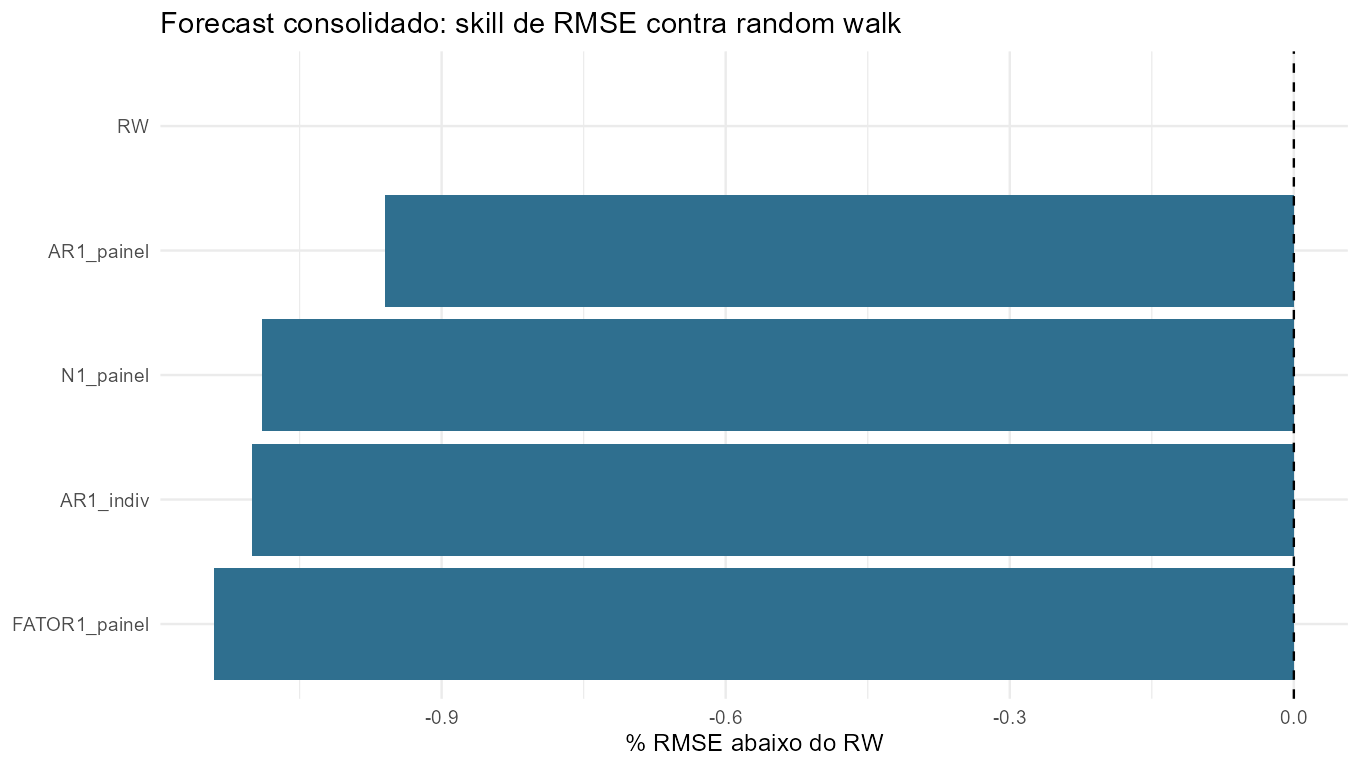
\includegraphics[width=0.82\textwidth]{forecast_consolidated_panel_skill.png}
\caption{Skill de RMSE no forecast consolidado contra random walk.}
\end{figure}

\section{CDA, grafos e duplicação}

\subsection{Por que a CDA continua no projeto}

A CDA continua porque responde a uma pergunta diferente da CONS. A CONS mede exposição final consolidada; a
CDA mostra a estrutura de cotas entre fundos. Ela é útil para risco, aninhamento, duplicação e extensão com
modelos de grafo.

\subsection{Ciclos e profundidade}

O subgrafo intra-amostra da CDA é DAG em todos os 72 meses. Portanto, não foram encontrados ciclos diretos
nas relações observadas. A profundidade máxima mediana é 7 e o máximo observado é 9, indicando camadas
relevantes de aninhamento.

\subsection{Duplicação intra-gestora}

Quando fundos da mesma gestora investem uns nos outros, somar exposições consolidadas por fundo pode contar
parte da exposição duas vezes. A de-duplicação usa:
\[
\phi_{A\to B}=\frac{valor_{A\to B}}{PL_B}
\]
e subtrai a fração da exposição de $B$ já carregada por $A$.

Para ITUB4, a duplicação intra-gestora estimada é 37,6\%. Esse número deve ser lido como duplicação
intra-gestora rastreável, não duplicação total do sistema.

\section{Auditoria e robustez}

A auditoria mestre está em \texttt{R/22\_master\_validation.R}. Ela transforma confiança em evidência
reprodutível. O resultado atual é:
\[
\text{PASS}=41,\qquad \text{FAIL}=0.
\]

Ela verifica:
\begin{itemize}
\item existência dos arquivos essenciais;
\item join CONS--SH;
\item tipo de ativo da CONS;
\item duplicatas dos painéis;
\item PTAX positiva;
\item reconstrução de quantidade por preço;
\item valores finitos;
\item CDA com CNPJ de destino, sem self-loop e sem valores negativos;
\item grafo acíclico;
\item outputs de forecasting;
\item separação entre núcleo CONS+SH e apêndice CDA.
\end{itemize}

Isso não garante que a CVM nunca tenha erro de origem. Garante que, dadas as bases e premissas do projeto, o
pipeline respeita as regras internas documentadas.

\section{Como explicar o projeto}

Uma explicação curta e correta:

\begin{quote}
O TCC constrói um painel mensal de exposição consolidada de gestoras brasileiras a ações usando CONS e SH da
CVM. A literatura de demand-based asset pricing motiva tratar carteiras institucionais como demanda
observada. O trabalho testa se a exposição futura pode ser prevista pelo histórico da própria gestora, pelo
restante do mercado e, em extensão, por redes de fundos. A CDA entra em apêndice para reconstruir a rede
fundo-sobre-fundo que a CONS apaga. O resultado final é que ITUB4 tem reversão à média em valor, mas no
painel amplo o random walk continua sendo o benchmark dominante.
\end{quote}

Uma explicação que deve ser evitada:

\begin{quote}
Estamos prevendo grafos.
\end{quote}

O correto é:

\begin{quote}
Estamos prevendo exposição consolidada; o grafo pode ser uma camada auxiliar de informação.
\end{quote}

\section{O que esperamos daqui para frente}

O resultado mais provável, se avançarmos para GNN, é que o ganho preditivo continue difícil. Há três razões:
\begin{enumerate}
\item o painel tem apenas 72 meses;
\item a feature manual de rede já não trouxe ganho;
\item o \emph{random walk} é muito forte para posições persistentes.
\end{enumerate}

Mesmo assim, uma GNN pode ser útil como extensão metodológica se for tratada corretamente. O critério é
simples: ela precisa ser comparada contra os baselines atuais e avaliada fora da amostra. Se não ganhar, o
resultado negativo deve ser reportado.

Para uma versão digna de SSRN, os próximos passos naturais são:
\begin{itemize}
\item limpar e fortalecer a redação em estilo paper;
\item confirmar a referência exata do working paper do orientador;
\item transformar tabelas principais em tabelas acadêmicas mais enxutas;
\item considerar uma versão em inglês;
\item discutir explicitamente limites de previsibilidade da demanda institucional;
\item manter a CDA como apêndice técnico ou extensão de rede, sem confundir com o núcleo CONS+SH.
\end{itemize}

\section{Conclusão}

O projeto está em uma posição melhor quando assume sua evidência com disciplina. A contribuição não é dizer
que encontramos uma máquina de prever demanda. A contribuição é construir uma base brasileira de exposição
institucional, validar cuidadosamente as unidades e joins, conectar essa base à literatura de demanda por
ações, documentar a estrutura de fundos sobre fundos via CDA e testar previsibilidade fora da amostra.

O achado final é:
\begin{quote}
Demanda institucional observada é mensurável e concentrada, mas sua previsibilidade mensal agregada é
limitada. Onde aparece sinal, ele é mais forte no nível patrimonial de blue chips específicas, como ITUB4,
do que na variação mensal ou no painel amplo de todas as ações.
\end{quote}

\bibliographystyle{plainnat}
\bibliography{refs}

\end{document}
